%%%%%%%%%%%%%%%%
%\chapter{Language Restrictions (Main Result: Theorems)}
%%%%%%%%%%%%%%%%

%State clearly definitions, assumptions, and proofs. The document will be archived for posterity and your name will be associated with any mistakes you make.

%%%%%%%%%%%%%%%%%%%%%%%%%%%%%%%%
\chapter{Design}
%%%%%%%%%%%%%%%%%%%%%%%%%%%%%%%%
% Introduce and discuss the design decisions that you made during this project.
% Highlight why individual decisions are important and/or necessary. Discuss
% how the design fits together.
% Use as much as needed.

The goal is to port Java to native restrictions with a minimal set of changes to the JDK. We want Java to behave exactly like Native Image, and crash for the exact same reasons that Native Image does. 
This section explains how semantic changes can be modeled through the concept of (1) native restrictions, (2) how defining scopes in the JDK enables us to express these changes, and (3) how we can improve Native Image usability by facilitating debugging of user code and identifying unexpected behaviour in Native Image by simulating it in Java.

%%%%%%%%%%%%%%%%%%%%%%%%%%%%%%%%
\section{Native Restrictions}
%%%%%%%%%%%%%%%%%%%%%%%%%%%%%%%%
We introduce the concept of native restrictions to represent the set of semantics that Java is running with. These restrictions modify the way dynamic class loading, reflection and the \verb|SecurityManager| behave at runtime. Each feature can be individually selected to run under native restrictions, it behaves like in Native Image, or not, it behaves like Java.
At the two end of the spectrum of the native restrictions, we have that: (1) when no restrictions are applied, Java behaves according to the Java Language Specification, (2) when all the restrictions are applied, Java behaves according to the Native Image Semantics, as presented in Section~\ref{native_image_specs}. 

At runtime, we perform checks for an expected behaviour depending on whether the feature is running under native restrictions or not, thus we effectively change the semantic of Java.
Moreover, proving that Java can behave like Native Image, while remaining compliant with the Java Compatibility Kit~\cite{noauthor_gaining_nodate}~(JCK), enables us to drive the specification of Native Image.

%%%%%%%%%%%%%%%%%%%%%%%%%%%%%%%%
\section{Native Restrictions Scopes}
%%%%%%%%%%%%%%%%%%%%%%%%%%%%%%%%
The challenge in designing the semantics changes is that they require us to differentiate runtime behavior from build time behavior - which is a concept that does not exist in Java - but also JVM calls from user calls on public methods.

One possible approach relies on bytecode transformation, but these transformations are both complex to implement and introduce non-trivial changes to the compiler. 
Instead, we use the notion of scopes to delimit regions of codes where the native restrictions are disabled. 
% This regions are explicitly delimited such that only code for the JVM is executed, arbitrary user-code remains restricted.
More formally, let \verb|c| be a method of the class or interface \verb|C|, and assume the existence of a mechanism to open scopes. As shown in Figure~\ref{fig:scopes}, \verb|c| opens a scope S, invokes a method \verb|a| of the class or interface \verb|A|, and closes S when it returns form \verb|a|.
The method \verb|a| invokes a method \verb|b| of the class or interface \verb|B| that performs some native restrictions checks.
Then if \verb|c| is invoked, the restrictions checks in \verb|b| will be ignored, as they are included in S.
If \verb|a| is invoked by another caller than \verb|C.c|, the restrictions checks in \verb|b| will be performed.

\begin{figure}[ht]
    \centering
\begin{lstlisting}[language=Java]
class A {
    static void a() {
        B.b(); 
    }
} 
class B {
    static void b() {
        // check native restrictions
    }
}
class C {
    static void c() {
       ...
       // start of scope S
       A.a();
       // end of scope S
       ...
    }
}
\end{lstlisting}
    \caption{Using scopes}
    \label{fig:scopes}
\end{figure}


In the following subsections we show in more details how these scopes were chosen for each feature, that they are correct according to Native Image semantics, and that the granularity of the scopes is optimal in the sense that delimiting another region would mean introducing more changes to the JDK for the design to remain correct.

%%%%%%%%%%%%%%%%%%%%%%%%%%%%%%%%
\subsection{Dynamic Class Loading}
%%%%%%%%%%%%%%%%%%%%%%%%%%%%%%%%
As mentioned in the background section, Native Image does not generally support dynamic class loading. The requirement under native restrictions are that loading a class at runtime without having registered it for reflection will result in a \verb|MissingReflectionRegistrationError| from \verb|java.lang.ClassLoader#defineClass1|, loading a class using a \verb|java.lang.invoke.MethodHandles.Lookup| invokes \verb|java.lang.ClassLoader#defineClass0| which will always throw an \verb|UnsupportedOperationException|.

The method \verb|java.lang.ClassLoader#loadClass| can be called from the JVM after a class has been linked, or directly from user-code. In the former case we do not want an exception to be thrown, in the latter case, we want to throw an exception to prevent user from defining an arbitrary class or interface at runtime.
% probably need to put that in the implementaiton ? the wrapper and everything
To differentiate these paths, we introduce the wrapper method \verb|java.lang.ClassLoader#runtimeLoadClass|. Instead of directly calling \verb|java.lang.ClassLoader#loadClass|, the JVM now calls the wrapper function. The JVM is also the only entry point, as shown in Figure~\ref{fig:load_class}.
Invoking \verb|runtimeLoadClass| opens a scope, which closes on \verb|defineClass1|'s return.
Since directly calling \verb|loadClass| does not open the scope, when \verb|defineClass1| is invoked, the native restrictions checks are still enabled, and a 
\verb|MissingReflectionRegistrationError| is thrown.

If not preloaded, then a class may be defined at runtime only if resolving the class or interface was required by one of the following instructions:
anewarray, checkcast, getfield, getstatic, instanceof, invokedynamic, invokeinterface, invokespecial,
invokestatic, invokevirtual, ldc, ldc\_w, multianewarray, new, putfield, and putstatic.
The wrapper then dispatches the call to the method loadClass to the delegate class loader, as intended when running without restrictions.
Runtime calls to the public method java.lang.ClassLoader#loadClass methods first checks if the class was preloaded (i.e. checking the inclusion of the class in the reflection metadata is sufficient to simulate Native Image behavior in this Java mode), before allowing it to be defined.

\begin{figure}
    \centering
    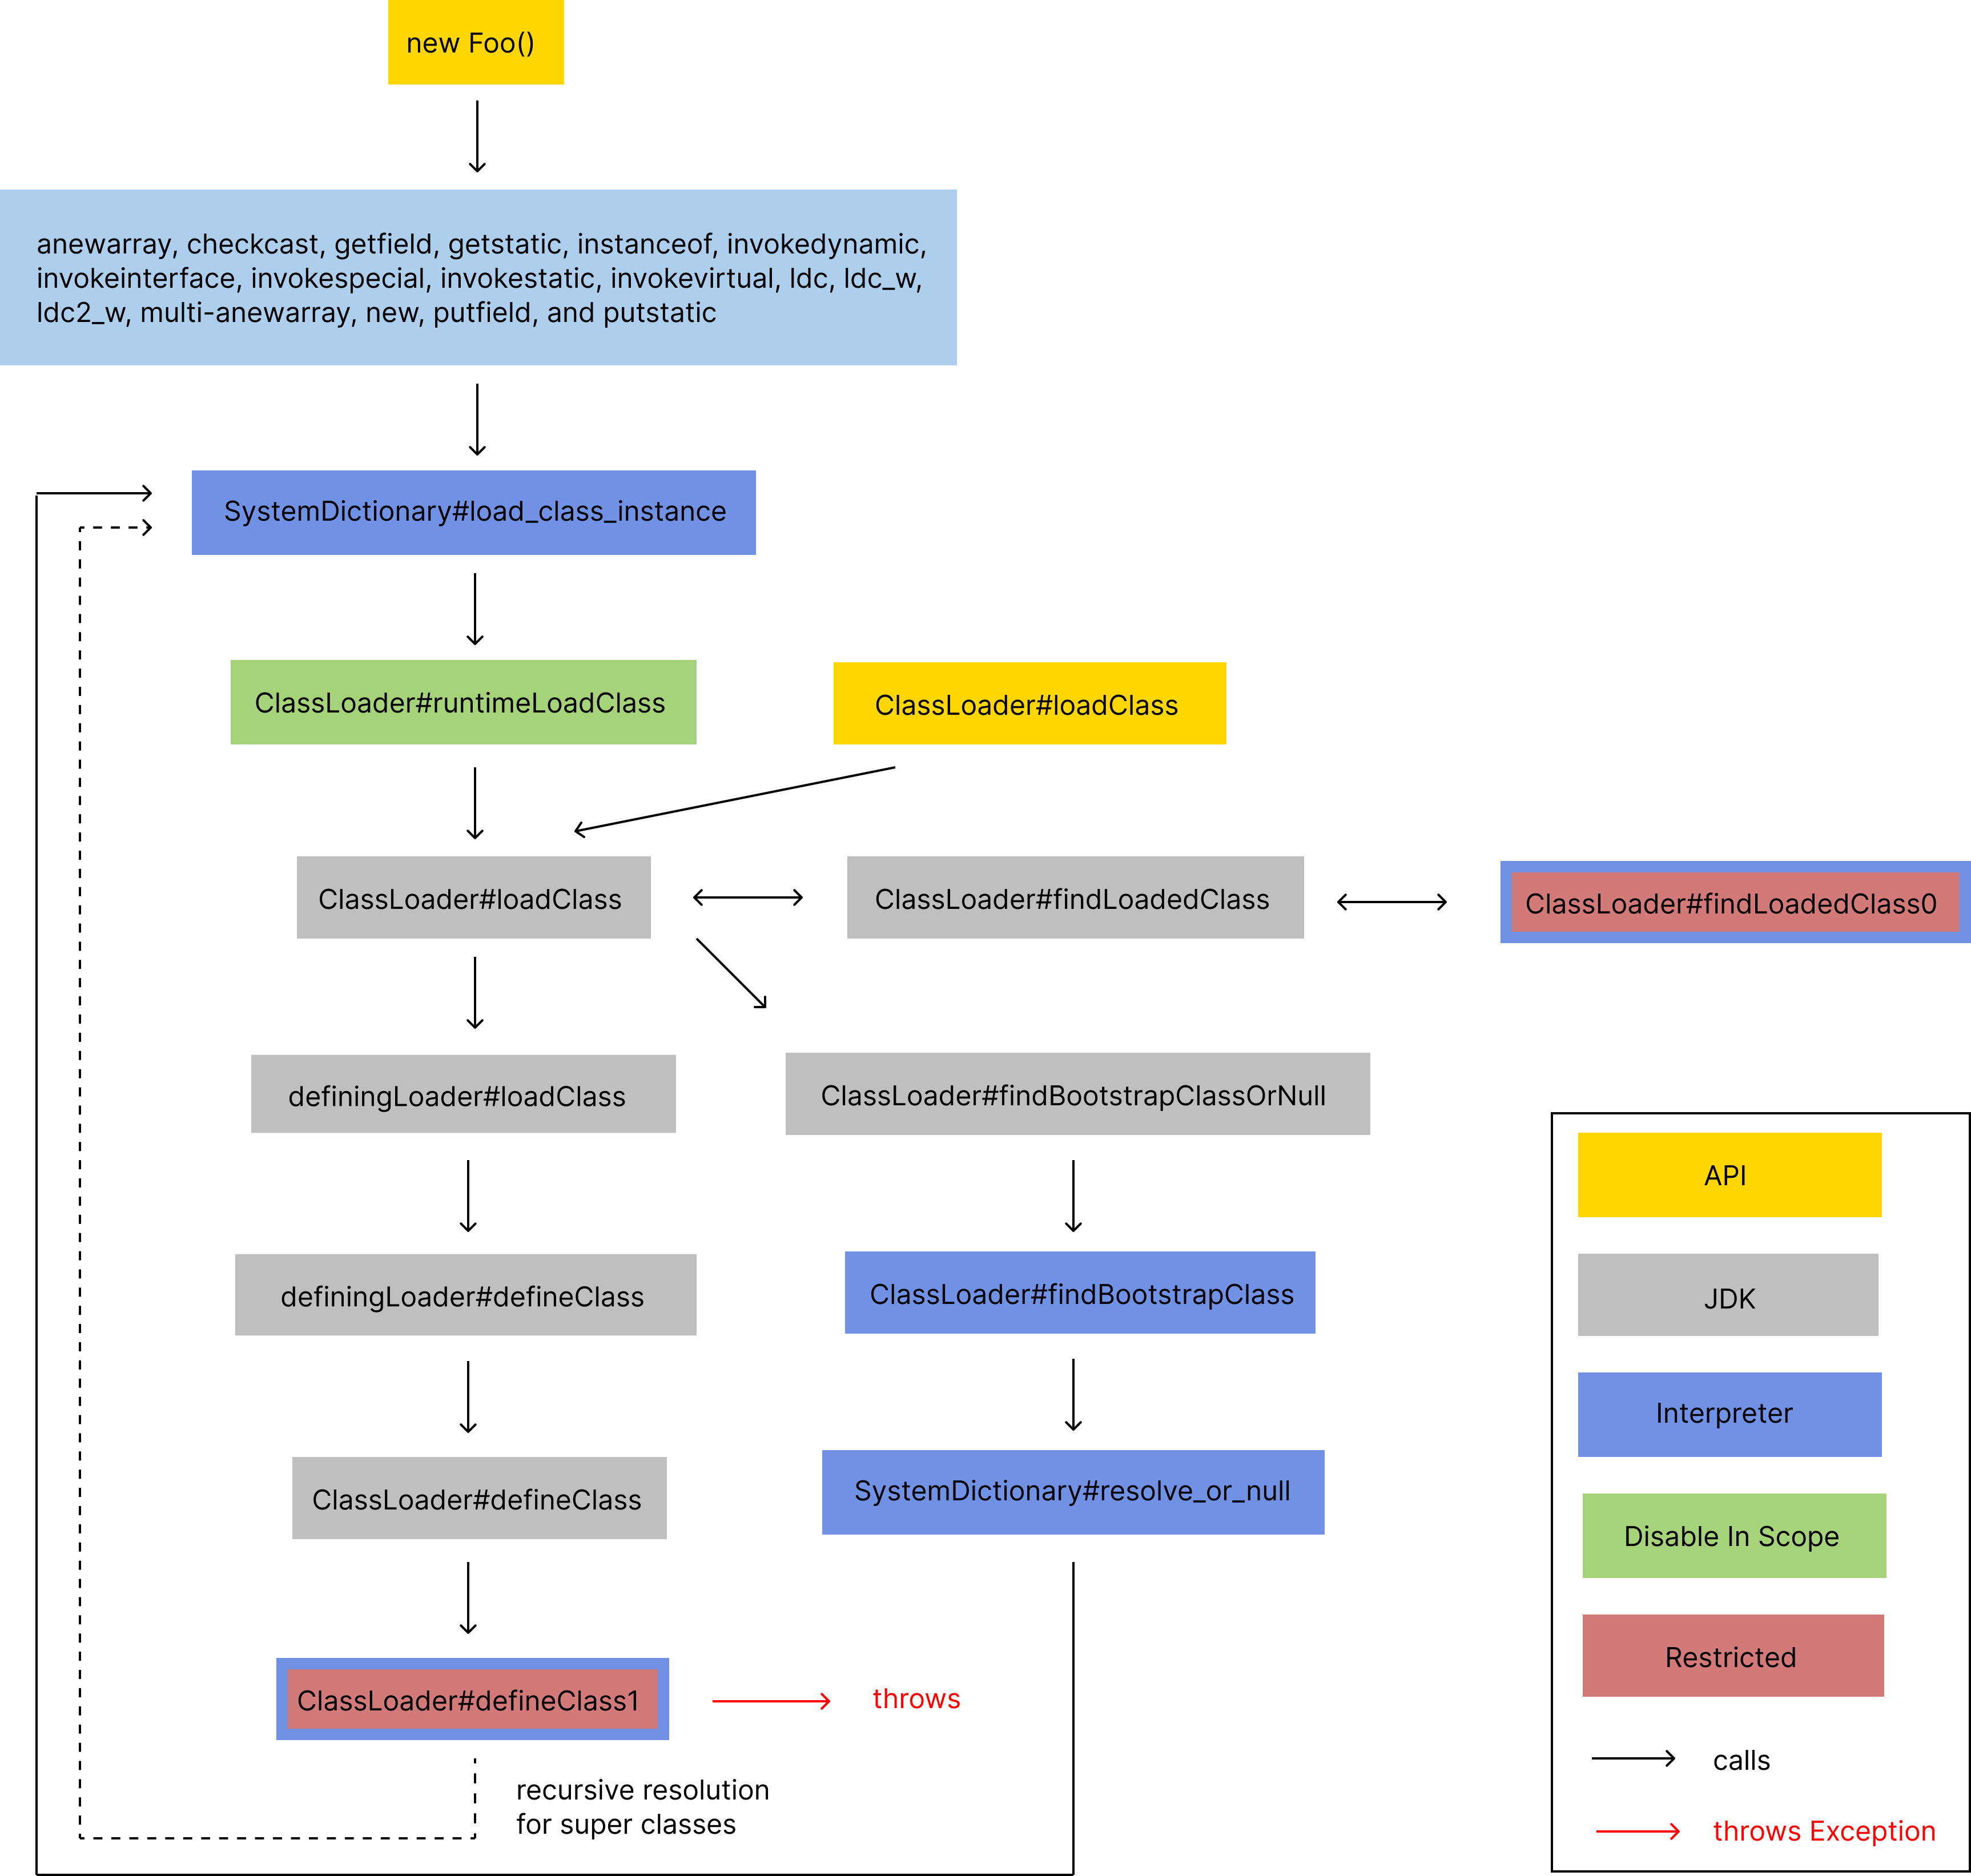
\includegraphics[scale=0.55]{resources/loadClassWithLegend.png}
    \caption{Caption}
    \label{fig:load_class}
\end{figure}


design flaw, when overloading the classloader, there's currently no way of knowing if a check has already been made for a class or not -> we check the metadata each time defineClass or findLoadedClass is called

Talk about all the other scopes that were introduced
See Appendix~\ref{minimal_change} for the full proof on the minimal changes.
%%%%%%%%%%%%%%%%%%%%%%%%%%%%%%%%
\subsection{Reflection}
%%%%%%%%%%%%%%%%%%%%%%%%%%%%%%%%
Introduce artificial checks for registration in all reflective access methods
Artificially use reflection for MemberName resolution -> bu since MemberName resolution is used all over the place by NethodHandles and all subclasses, then we must also introduce scopes to preventthe checks for internal classes.
%%%%%%%%%%%%%%%%%%%%%%%%%%%%%%%%
\section{Improving Usability}
%%%%%%%%%%%%%%%%%%%%%%%%%%%%%%%%

%%%%%%%%%%%%%%%%%%%%%%%%%%%%%%%%
\subsection{Say Goodbye to GDB}
%%%%%%%%%%%%%%%%%%%%%%%%%%%%%%%%
Native Image offers a tracing agent to automatically collect the reachability metadata required for an application
A new workflow for building an image.
- run the agent, run the java mode, debug with java, build your image
%%%%%%%%%%%%%%%%%%%%%%%%%%%%%%%%
\subsection{Defining unexpected behavior}
%%%%%%%%%%%%%%%%%%%%%%%%%%%%%%%%
Put list of bugs here!
This one does not throw:
public class Main {
    public static void main(String[] args) throws Exception {
        Class<?> cl = Class.forName("pfoo.PackageFoo");
    }
}

But then this one does
public class Main {
    public static String hideLiterals(String s) {
        System.out.println();
        return s;
    }
    public static void main(String[] args) throws Exception {
        Class<?> cl = Class.forName(hideLiterals("pfoo.PackageFoo"));
    }
}

This one does not throw:
package foo;
public class Foo {
    public String toString() {
        return "Hello There " + message;
    }
}
public static void testFindVirtual(MethodHandles.Lookup lookup) throws Throwable {
    String methodName = "toString";
    MethodHandle mh = lookup.findVirtual(Foo.class, hideLiterals(methodName), mt(String.class));
}
This one does
package foo;
public class FooLoader extends ClassLoader {
    @Override
    public Class<?> loadClass(String name) throws ClassNotFoundException {
        return super.loadClass(name);
    }
}
public static void testLoadClassBindCaller(MethodHandles.Lookup lookup) throws Throwable {
    MethodHandle mh = lookup.findVirtual(FooLoader.class, "loadClass", mt(Class.class, String.class));
}

Always hide the parameters behind a method call that can't be inlined or it doesn't throw


Defining class: Avoid bytecode rewriting -> create a loadClass wrapper instead, to differentiate users from the interpreters call
Balance between what needs to be changed in Native Image, driving the specs with this Java mode, and using part of what is in Nativ eImage in Java mode (e.g. 
MissingReflectionRegistrationError is still in progress in Native Image, but also using in Java).

Building the agent after doing the defineClass -> back and forth
SecurityManager was changed in Java moide, so had to change in NI, but other changes were made in NI so also had to propagate back the changes into the Java mode.
etc.


%%%%%%%%%%%%%%%%%%%%%%%%%%%%%%%%
\chapter{Implementation}
%%%%%%%%%%%%%%%%%%%%%%%%%%%%%%%%
% The implementation covers some of the implementation details of your project.
% This is not intended to be a low level description of every line of code that
% you wrote but covers the implementation aspects of the projects.
% Please provide as stable as possible links to the implementation source code.
A mix of software archeology and software surgery.
LanguageRestrictions, Restrictions bundles and restrictions


%%%%%%%%%%%%%%%%%%%%%%%%%%%%%%%%
\section{LanguageRestrictionManager}
%%%%%%%%%%%%%%%%%%%%%%%%%%%%%%%%


%%%%%%%%%%%%%%%%%%%%%%%%%%%%%%%%
\section{Native Restrictions Scopes}
%%%%%%%%%%%%%%%%%%%%%%%%%%%%%%%%
Concretely scopes are thread locals of integers, basically counters!
Each time a region is entered, the counter is incremented, and each time a region is left, the counter is decremented. This account for recursive calls (they either all get disabled or all enabled).

To avoid memory leak, the thread local is instantiated in a try-catch clause, and implement the autocloasable interface.
To minimize changes made to the JDK, the try catch clause is hidden in a Lambda whenever possible (i.e. StackOverflow can happen when the region is located in part of the JDK used to bootstrap lambdas).


%%%%%%%%%%%%%%%%%%%%%%%%%%%%%%%%
\section{Class Loader}
%%%%%%%%%%%%%%%%%%%%%%%%%%%%%%%%
Native Image does not allow for runtime definition of classes that were not preloaded beforehand.
To simulate this behavior, we introduce the wrapper method java.lang.ClassLoader#runtimeLoadClass. The only entry point for this private method is the interpreter. If not preloaded, then a class may be defined at runtime only if resolving the class or interface was required by one of the following instructions:
anewarray, checkcast, getfield, getstatic, instanceof, invokedynamic, invokeinterface, invokespecial,
invokestatic, invokevirtual, ldc, ldc\_w, multianewarray, new, putfield, and putstatic.
The wrapper then dispatches the call to the method loadClass to the delegate class loader, as intended when running without restrictions.
Runtime calls to the public method java.lang.ClassLoader#loadClass methods first checks if the class was preloaded (i.e. checking the inclusion of the class in the reflection metadata is sufficient to simulate Native Image behavior in this Java mode), before allowing it to be defined.

\begin{lstlisting}[language=Java]
private Class<?> runtimeLoadClass(String name) throws ClassNotFoundException {
    try(ClassLoaderDefineClass unused = ClassLoaderLoaderDefineClass .setIsRuntimeDefineClassAllowed()) {
        return this.loadClass(name);
    }
}
\end{lstlisting}

TODO add a simple running example: in one case creating an object new Foo() -> intepreter call
in another loadong the class foo with and without preloading

Do an upcall in native code in ClassLoader.c to check if the dynamicClassLoading is restricted or not and throw an UnsupportedOperationException is so.

%%%%%%%%%%%%%%%%%%%%%%%%%%%%%%%%
\section{Invoke dynamic}
%%%%%%%%%%%%%%%%%%%%%%%%%%%%%%%%
Talk about BMI, and how certain BMI are allowed and other not, as well as restricting the LambdaMetafactory
Use lambda to surround and hide the checks

%%%%%%%%%%%%%%%%%%%%%%%%%%%%%%%%
\section{Reflection}
%%%%%%%%%%%%%%%%%%%%%%%%%%%%%%%%
don't want to trace internal classes!
> first implementation of the restrict for LambdaMetafactory and the BMI was too restrictive,
i.e. only allowed LambdaMEtfactory all other bsmethod where restricted, which is not correct ->
checked NI and try to get as close as possible, it executes some safe bsmethods at build time and
the rest is interpreted at runtime -> basically only lambda and other System class are allowed in
Java mode, if the user tries to do something strange (assuming they haven’t overriden the App class
loader), then either the call site must have been preloaded before, or it will throw when it tries to
resolve the method name

%%%%%%%%%%%%%%%%%%%%%%%%%%%%%%%%
\section{Tracing agent}
%%%%%%%%%%%%%%%%%%%%%%%%%%%%%%%%

Have everything in one place -> simple work flow run the agent test with java under native restrictions adn then build the image -> don't need to build graalvm before

%%%%%%%%%%%%%%%%%%%%%%%%%%%%%%%%
\section{Unimplemented feature: Security Manager}
%%%%%%%%%%%%%%%%%%%%%%%%%%%%%%%%
-> Throws a VMError fatal error, cannot be catched
-> instead

%%%%%%%%%%%%%%%%%%%%%%%%%%%%%%%%
\section{Technology Compatibility Kit}
%%%%%%%%%%%%%%%%%%%%%%%%%%%%%%%%
An experience in meta-programming. 
Gradle project designed to compile with an annotation processor. Parses all @Test annotation and write the json configuration for each test on the fly
during compilation.
Test harness run all test that implements the TestProvider class. Single test per file
The reflection configurations are not on the classpath on purpose. There's a flag in NI and Java so that the path to the reflection configurations files can be specified.
-> Build two native images, one with the reflection and another without. Run with Java with and without the reflection configuration path specified as a sys prop.

-> the TCK is an implementation/represents of the specs of native image
-> it's a simple random bug catcher, 
\url{https://en.wikipedia.org/wiki/Programming_language_specification}
Semantics

Formulating a rigorous semantics of a large, complex, practical programming language is a daunting task even for experienced specialists, and the resulting specification can be difficult for anyone but experts to understand. The following are some of the ways in which programming language semantics can be described; all languages use at least one of these description methods, and some languages combine more than one[5]

    Natural language: Description by human natural language.
    Formal semantics: Description by mathematics.
    Reference implementations: Description by computer program
    Test suites: Description by examples of programs and their expected behaviors. While few language specifications start off in this form, the evolution of some language specifications has been influenced by the semantics of a test suite (e.g. in the past the specification of Ada has been modified to match the behavior of the Ada Conformity Assessment Test Suite).

%%%%%%%%%%%%%%%%%%%%%%%%%%%%%%%%
\chapter{The Native Image Specification}\label{native_image_specs}
%%%%%%%%%%%%%%%%%%%%%%%%%%%%%%%%
%% TODO add snippets of code to show how it differes from normal Java
# Native Image Semantics

Native Image operates under a closed-world assumption. This assumption affects the semantics of the 
Java® programming language as defined in the 
[Java Language Specification](https://docs.oracle.com/javase/specs/jls/se21/html/index.html).
We refer to this set of semantics as Native Image semantics, and is strictly equivalent to running
Java under native restrictions.

This document specifies the semantics of Native Image.
It is organised according to the following sections:
* [Reflection](#reflection)
* [Resources](#resources)
* [Serialization](#serialization)
* [Dynamic Class Loading](#dynamic-class-loading)
* [Misc.](#misc)

# Reflection
Under native restrictions, every reflectively-accessed element, that is `Class`, `Executable`, and `Field`, must 
be included in the reflection metadata (see [Specifying Reflection Metadata in JSON](https://www.graalvm.org/latest/reference-manual/native-image/metadata/#specifying-reflection-metadata-in-json)
for more details). If the element is not registered for reflection, then a `MissingReflectionRegistrationError` is thrown.

### Reflectively-Accessing a Class
Calling `java.lang.Class#forName` for a class or interface C requires C to be registered for reflection.
If C is registered, and C cannot be located, then a `ClassNotFoundException` is thrown. 
Superclasses of C are not automatically registered for reflection if C is registered.

Creating a new array of component type C using `java.lang.reflect.Array#newInstance` requires C to be 
registered for reflection.

Instantiating C with the method `sun.misc.Unsafe#allocateInstance` requires C to be 
registered for reflection and the flag `unsafeAllocated` must be set to true.

### Reflectively-Accessing a Method
Calling `java.lang.Class#getMethod` and `java.lang.Class#getDeclaredMethod` on a class or interface C for a method M, 
with parameters of types T<sub>1</sub>...T<sub>n</sub>, require C, M and T<sub>1</sub>...T<sub>n</sub> to be registered 
for reflection.
If M is registered, but M cannot be found, then a `NoSuchMethodException` is thrown.

Invoking the method M of C using `java.lang.reflect.Method#invoke` requires C to be registered for reflection
and M to be registered as accessed in the reflection metadata.
A `MissingReflectionRegistrationError` is thrown if C or M is not registered for reflection, or 
if M is only registered as being queried.

### Reflectively-Accessing a Constructor
Calling `java.lang.Class#getConstructor` and `java.lang.Class#getDeclaredConstructor` on a class or interface C 
for a constructor N with parameters of types T<sub>1</sub>...T<sub>n</sub>, require C, M and T<sub>1</sub>...T<sub>n</sub>
to be registered for reflection,
If N is registered, but N cannot be found, then a `NoSuchMethodException` is thrown.

Creating a new instance of the class or interface C using the constructor N using
`java.lang.reflect.Constructor#newInstance` requires C to be registered for reflection
and N to be registered as accessed in the reflection metadata.
A `MissingReflectionRegistrationError` is thrown if C or N is not registered for reflection, or
if N is only registered as being queried.

### Reflectively-Accessing a Field
Calling `java.lang.Class#getField` and `java.lang.Class#getDeclaredField` on a class or interface C for a field F,
require the C and F to be registered for reflection.
If F is registered for reflection, but F cannot be found, then a `NoSuchFieldException` is thrown.

### Reflectively-Accessing Member Classes and Interfaces
When called on the class or interface C, the following methods require C to be registered for reflection with
a specific flag set:
* `java.lang.Class#getClasses` along with the flag `allPublicClasses` set to true
* `java.lang.Class#getDeclaredClasses` along with the flag `allDeclaredClasses` set to true

### Reflectively-Accessing the Methods of a Class
When called on the class or interface C, the following methods require C to be registered for reflection with 
a specific flag set:
* `java.lang.Class#getMethods` along with the flag `allPublicMethods` set to true
* `java.lang.Class#getDeclaredMethods` along with the flag `allDeclaredMethods` set to true

### Reflectively-Accessing the Constructors of a Class
When called on the class or interface C, the following methods require C to be registered for reflection with
a specific flag set:
* `java.lang.Class#getConstructors` along with the flag `allPublicMethods` set to true
* `java.lang.Class#getDeclaredConstructors` along with the flag `allDeclaredMethods` set to true

### Reflectively-Accessing the Fields of a Class
When called on the class or interface C, the following methods require C to be registered for reflection with
a specific flag set:
* `java.lang.Class#getFields` along with the flag `allPublicFields` set to true
* `java.lang.Class#getDeclaredFields` along with the flag `allDeclaredFields` set to true

### Reflectively-Accessing the Permitted Subclasses of a Class
Calling `java.lang.Class#getPermittedSubclasses` on a class or interface C requires C to be registered for reflection
and its flag `allPermittedSubclasses` to be set to true.

### Reflectively-Accessing the Nest Members of a Class
Calling `java.lang.Class#getNestMembers` on a class or interface C requires C to be registered for reflection 
and its flag `allNestMembers` to be set to true.

### Reflectively-Accessing the Record Components of a Class
Calling `java.lang.Class#getRecordComponents`on a class or interface C requires C to be registered for reflection
and its flag `allRecordComponents` to be set to true.

### Reflectively-Accessing the Signers of a Class
Calling `java.lang.Class#getSigners`on a class or interface C requires C to be registered for reflection
and its flag `allSigners` to be set to true.

## Resources
## Serialization

## Dynamic Class Loading
In this section, we explain the differences that occur during the process of dynamically loading
a class or interface at runtime under native restrictions. 
If not explicitly specified, then a call to a method refers to a call from the API, 
rather than an internal calls.

### Class and Interface Resolution
Under native restrictions, the following rules apply: 
* All classes from the classpath are linked before the execution of the program
* All `invokedynamic` instructions are resolved at build time before program execution and replaced
  with adequate bytecodes

A class or interface dynamically loaded at runtime must be registered for reflection.

If the element is not registered, then:
* Calling any of the declared methods `loadClass` of `java.lang.ClassLoader` will result in a 
`MissingReflectionRegistrationError`.
* Calling any method of a user-defined class loader that depends on the methods `java.lang.ClassLoader#loadClass`, 
`java.lang.ClassLoader#findLoadedClass` or `java.lang.ClassLoader#findBootstrapClassOrNull` 
will result in a `MissingReflectionRegistrationError`.

If the element is registered, then resolution proceeds as described in 
[Section 5.4.3. of the JLS](https://docs.oracle.com/javase/specs/jvms/se21/html/jvms-5.html#jvms-5.4.3).

### Method Handle Resolution
Unless they are used as part of the `invokedynamic` instruction, calls to the following methods 
will result in an `UnsupportedOperationException`:
* `java.lang.invoke.MethodHandles.Lookup#defineClass`
* `java.lang.invoke.MethodHandles.Lookup#defineHiddenClass`
* `java.lang.invoke.MethodHandles.Lookup#defineHiddenClassWithClassData`

### java.lang.invoke.LambdaMetafactory
Unless they are used as part of the `invokedynamic` instruction, calls to `java.lang.invoke.LambdaMetafactory#metafactory` 
and `java.lang.invoke.LambdaMetafactory#altMetafactory` will result in an `UnsupportedOperationException`.


## Unimplemented Features
#### java.lang.SecurityManager
The `java.lang.SecurityManager` behaves in the following ways:
* `java.lang.System#getSecurityManager()` always returns `null`
* `java.lang.System#setSecurityManager(SecurityManager sm)` returns without exception if `sm` is null. 
It throws a `SecurityException` if the system property `java.security.manager` is not set to `disallow`, and an 
`UnsupportedOperationException` otherwise.



%%%%%%%%%%%%%%%%%%%%%%%%%%%%%%%%
% \chapter{Evaluation}
%%%%%%%%%%%%%%%%%%%%%%%%%%%%%%%%

% In the evaluation you convince the reader that your design works as intended.
% Describe the evaluation setup, the designed experiments, and how the
% experiments showcase the individual points you want to prove.

